\documentclass[aspectratio=169,11pt]{beamer}
\usepackage[utf8]{inputenc}
\usepackage[T1]{fontenc}
\usepackage[english]{babel}
\usepackage{amsmath,amssymb}
\usepackage{graphicx}
\usepackage{booktabs}

\usetheme{Madrid}
\usecolortheme{default}

\title{Clasificador bayesiano generativo\\para d\'igitos MNIST}
\subtitle{Probabilidad y Estad\'istica --- Proyecto final}
\date{}

\begin{document}

% ---- Slide 1: Problema ----
\begin{frame}{Problema}
\begin{block}{?`Qu\'e quiero construir?}
Una funci\'on que reciba una imagen y devuelva una clase:
\[
  f(x) = \hat{y}, \qquad x\in\mathbb{R}^{784},\quad
  y\in\{0,1,\dots,9\}.
\]
\end{block}

\begin{block}{Regla de decisi\'on}
Escogemos la clase m\'as probable:
\[
  \hat{y} = \arg\max_{c\in\{0,\dots,9\}} P(y=c\mid x)
\]
\end{block}

\begin{block}{Teorema de Bayes}
\[
  P(y=c\mid x) = \frac{P(y=c)\;p(x\mid y=c)}{p(x)}
  \quad\Longrightarrow\quad
  \hat{y} = \arg\max_c \bigl[\log P(y=c) + \log p(x\mid y=c)\bigr]
\]
\end{block}
\end{frame}

% ---- Slide 2: Metodolog\'ia ----
\begin{frame}{Metodolog\'ia}
\begin{block}{Suposici\'on: distribuci\'on normal multivariada}
\[
  x\mid y=c \;\sim\; \mathcal{N}(\mu_c,\,\Sigma_c)
\]
\end{block}

\begin{block}{Par\'ametros estimados por m\'axima verosimilitud}
\[
  \hat{P}(y=c) = \frac{N_c}{N}, \qquad
  \hat{\mu}_c = \frac{1}{N_c}\sum_{i:\,y_i=c} x_i, \qquad
  \hat{\Sigma}_c = \frac{1}{N_c}\sum_{i:\,y_i=c}
    (x_i-\hat{\mu}_c)(x_i-\hat{\mu}_c)^{\mathsf{T}}
\]
\end{block}

\begin{block}{Regla de clasificaci\'on final}
\[
  \hat{y} = \arg\max_c \Bigl[
    \log \hat{P}(y=c)
    - \tfrac{1}{2}\log|\hat{\Sigma}_c|
    - \tfrac{1}{2}(x-\hat{\mu}_c)^{\mathsf{T}}
      \hat{\Sigma}_c^{-1}(x-\hat{\mu}_c)
  \Bigr]
\]
\end{block}

Regularizaci\'on: $\hat{\Sigma}_c^{\,\text{reg}} = \hat{\Sigma}_c +
\varepsilon\,\mathbf{I}_d$, \; $\varepsilon = 10^{-4}$.
\end{frame}

% ---- Slide 3: Gr\'aficos principales ----
\begin{frame}{Gr\'aficos principales}
\begin{columns}[T]
\begin{column}{0.48\textwidth}
  \centering
  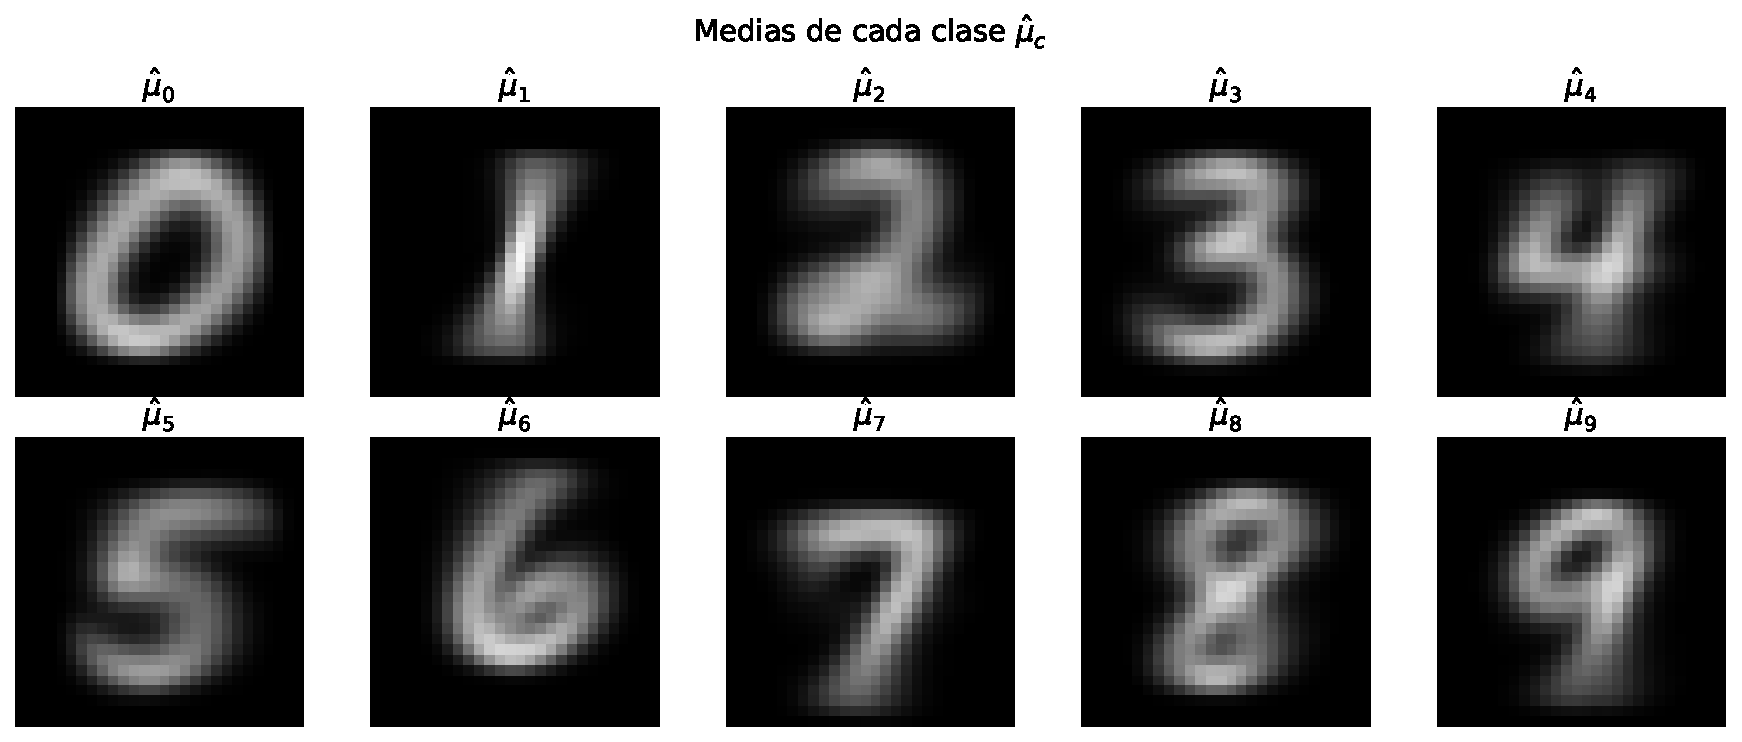
\includegraphics[width=\textwidth]{figs/means.pdf}\\[4pt]
  {\small Medias de cada clase $\hat{\mu}_c$}
\end{column}
\begin{column}{0.48\textwidth}
  \centering
  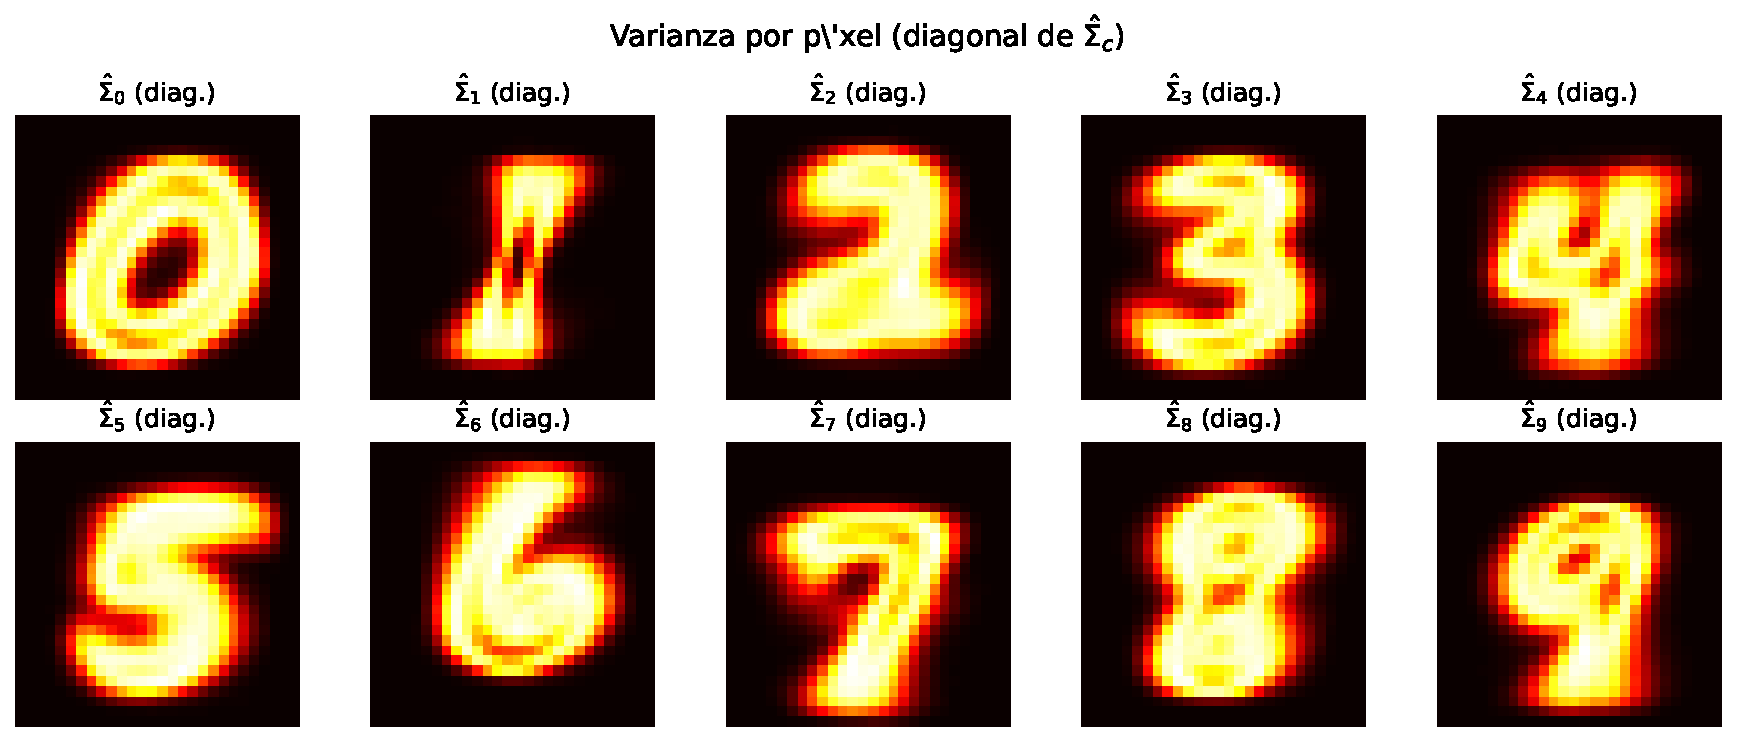
\includegraphics[width=\textwidth]{figs/cov_diag.pdf}\\[4pt]
  {\small Varianza por p\'ixel (diagonal de $\hat{\Sigma}_c$)}
\end{column}
\end{columns}
\end{frame}

% ---- Slide 4: Resultados ----
\begin{frame}{Resultados}
\begin{itemize}
  \item Exactitud global: $86{,}55\,\%$
  \item D\'igitos m\'as confusos: 5 y 7
  \item El modelo separa bien los d\'igitos con forma m\'as
        distintiva (0, 1, 6)
\end{itemize}

\vspace{0.5em}
\centering
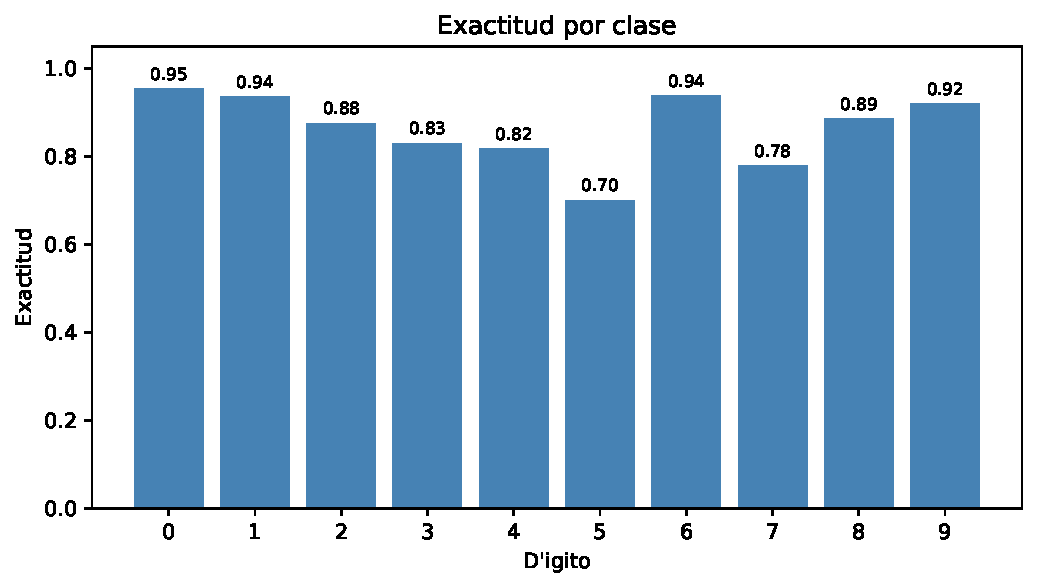
\includegraphics[width=0.72\textwidth]{figs/per_class_acc.pdf}
\end{frame}

% ---- Slide 5: Conclusiones ----
\begin{frame}{Conclusiones}
\begin{enumerate}
  \item Construimos un \textbf{clasificador bayesiano generativo} que modela
        $p(x\mid y=c)$ como una normal multivariada para cada d\'igito.

  \item Los par\'ametros se estiman por m\'axima verosimilitud
        \textbf{sin necesidad de optimizaci\'on iterativa}.

  \item La interfaz probabil\'istica permite cuantificar la
        \textbf{confianza} en cada predicci\'on, no solo dar la clase
        predicha.

  \item La exactitud del $86{,}55\,\%$ es razonable para un modelo
        generativo simple sin redes neuronales.

  \item Las matrices de covarianza muestran que el modelo captura la
        estructura de p\'ixeles de cada d\'igito.
\end{enumerate}
\end{frame}

\end{document}
